\documentclass[twocolumn]{article}

\usepackage{arxiv}

% ------------------------------------------------------------------ layout
% arxiv.sty is single-column with 1in side margins; for two columns we use
% 0.75in margins and a 0.25in gutter (applied after arxiv.sty's own geometry).
\AtBeginDocument{%
  \newgeometry{letterpaper,left=0.75in,right=0.75in,top=0.9in,bottom=0.9in,
               headheight=14pt,headsep=16pt,footskip=26pt}%
  \setlength{\columnsep}{0.25in}%
}
\raggedbottom   % arxiv.sty uses \flushbottom, which stretches gaps in two columns

% ------------------------------------------------------------------ packages
\usepackage[utf8]{inputenc}
\usepackage[T1]{fontenc}
\usepackage{amsmath}
\usepackage{newtxtext,newtxmath}
\usepackage{bm}
\usepackage{microtype}
\usepackage{graphicx}
\usepackage{booktabs}
\usepackage{tabularx}
\usepackage{array}
\usepackage{xcolor}
\usepackage[font=small,labelfont=bf,skip=4pt]{caption}
\usepackage{enumitem}
\usepackage{algorithm}
\usepackage{algpseudocode}
\usepackage{tikz}
\usepackage{placeins}
\usepackage[numbers,sort&compress]{natbib}
\usepackage[hidelinks]{hyperref}
\usepackage{url}

\setlist{nosep,leftmargin=1.2em}
\setlength{\textfloatsep}{10pt plus 2pt minus 2pt}
\setlength{\dbltextfloatsep}{10pt plus 2pt minus 2pt}
\setlength{\floatsep}{8pt plus 2pt minus 2pt}
\renewcommand{\arraystretch}{1.1}

% ------------------------------------------------------------------ macros
\newcommand{\R}{\mathbb{R}}
\newcommand{\E}{\mathbb{E}}
\newcommand{\ind}{\mathbf{1}}
\newcommand{\cfg}[1]{\texttt{#1}}
\newcommand{\pend}{\textcolor{gray}{tbd}}
\newcommand{\todo}[1]{\textcolor{orange!80!black}{\emph{[#1]}}}

% Include figures/<file> if it exists, otherwise draw a labelled placeholder.
\newcommand{\resultfig}[3][\linewidth]{%
  \IfFileExists{figures/#2}{%
    \includegraphics[width=#1]{figures/#2}%
  }{%
    \fbox{\parbox[c][#3][c]{\dimexpr#1-2\fboxsep-2\fboxrule}{\centering\small\textcolor{gray}{%
      Figure pending (main sweep): \texttt{figures/\detokenize{#2}}}}}%
  }%
}

% ------------------------------------------------------------------ title
\renewcommand{\headeright}{CS 329 Final Report}
\renewcommand{\undertitle}{CS 329: Foundations of AI --- Multiagent Systems \quad$\cdot$\quad Final Project Report}
\renewcommand{\shorttitle}{Communication-Constrained MARL}

\title{How Many Messages Does a Team Need?\\[2pt]
\large Communication-Efficient Coordination in a Rocket League-Inspired Environment}

\author{%
  Aryan Kumar \\ \texttt{aryan.kumar@iitgn.ac.in}
  \And
  Rayan Talukder \\ \texttt{rayan.talukder@iitgn.ac.in}
  \AND
  Swami Aryanathan Gantedi \\ \texttt{gantedi.aryanathan@iitgn.ac.in}
  \And
  Kudumula Vinod Kumar Reddy \\ \texttt{vinod.kudumula@iitgn.ac.in}
  \AND
  \normalfont Department of Computer Science, IIT Gandhinagar \quad$\cdot$\quad
  \url{https://github.com/AceAryan/marl-rocket}
}
\date{}

\begin{document}

\twocolumn[{%
\maketitle
\vspace{-0.4in}
\begin{abstract}
Cooperating agents rarely have free communication: bandwidth is limited and every message costs
energy. We ask how much communication two reinforcement-learning teammates actually need. In a 2D
soccer task inspired by Rocket League, two independent Double-DQN agents see only a small radius around
themselves, a goal counts only if the teammate assisted it, and each agent may send a limited number
of messages per episode carrying what it currently sees. Comparing a fixed broadcast schedule, a
hand-coded rule and a learned sender, which decides when to send using counterfactual rollouts of the
game, we separate the value of the information from the skill of choosing when to share it. Getting
there took six versions of the environment and learner and 1\,213 training runs. For most of them
communication showed no benefit, which we traced to a hidden free channel, a flawed credit signal and
a task that was too easy. A pre-registered pilot then fixed the regime for a main sweep of 580 runs
over the message budget, delay and view radius, from which we estimate the budget at which
communication saturates.
\end{abstract}
\keywords{multi-agent reinforcement learning \and communication budgets \and partial observability
\and independent Q-learning \and difference rewards}
\vspace{0.2in}
}]

% =====================================================================
\section{Introduction}
% =====================================================================

Platoons of vehicles, warehouse robots and sensor networks all coordinate under limits on how much
they can say to each other~\citep{weiss2000,zhang2013}. Work on learned communication in multi-agent
reinforcement learning (MARL), such as CommNet~\citep{sukhbaatar2016}, RIAL/DIAL~\citep{foerster2016}
and IC3Net~\citep{singh2019}, has mostly asked \emph{what} agents should say. We ask a more
practical question: \emph{how much} must they say? If a team keeps most of its performance with a
handful of messages, an engineer can budget bandwidth accordingly.

We study this in a deliberately simple setting. Two agents play a 2D soccer task where neither can
see far, so each depends on the other to find the ball. Messages are useful but rationed. Three
questions guide the study:
\begin{itemize}
\item \textbf{RQ1 (saturation).} As the per-episode budget $B$ grows from $0$ to $\infty$, where does
the team stop improving?
\item \textbf{RQ2 (delay).} How much does a delivery delay $\delta$ erode the value of messages?
\item \textbf{RQ3 (observability).} Does communication matter more when agents see less?
\end{itemize}

Our contributions are: (i) an environment in which messages carry decision-relevant information that
cannot leak through any other channel; (ii) a learned sender credited by \emph{counterfactual
rollouts}, which price each message against the budget it uses up; (iii) a comparison of learned,
rule-based and fixed-schedule senders that separates what a message says from when it is sent; and
(iv) a record of six design iterations, including the failures, followed by a pre-registered pilot.

% =====================================================================
\section{Background}
% =====================================================================

\textbf{Dec-POMDP with a channel.} $n=2$ agents act on local observations $o^i_t$ and share a reward
$r_t$~\citep{oliehoek2016}. Besides its action $a^i_t$, agent $i$ may send a message, which the
teammate receives at step $t+\delta$. The budget $B$ caps the messages each agent sends per episode:
\begin{equation}
\max_{\pi^1,\pi^2}\ \E\Big[\sum_{t=0}^{T}\gamma^t r_t\Big]
\ \ \text{s.t.}\ \ \sum_{t=0}^{T}\ind[m^i_t\neq\varnothing]\le B\ \ \forall i.
\end{equation}

\textbf{Independent Double DQN.} Each agent learns its own Q-network~\citep{watkins1992,mnih2015},
treating the teammate as part of the environment (independent Q-learning, IQL~\citep{tan1993}).
We use Double DQN~\citep{vanhasselt2016} with $n$-step returns~\citep{sutton2018}:
\begin{equation}
y_t=\sum_{k=0}^{n-1}\gamma^k r_{t+k}+\gamma^n Q_{\bar\theta}\big(o_{t+n},\textstyle\arg\max_{a}Q_\theta(o_{t+n},a)\big).
\label{eq:ddqn}
\end{equation}
IQL has no convergence guarantee, because the teammate keeps changing, but it is the simplest fully
decentralised baseline; centralised methods such as QMIX~\citep{rashid2018} are left for future work.

\textbf{Difference rewards.} The credit for one agent's choice can be measured as the change in
team return when only that choice is changed~\citep{wolpert2002}. We use this to judge whether a
message was worth sending.

% =====================================================================
\section{Environment}\label{sec:env}
% =====================================================================

\begin{figure}[!t]
\centering
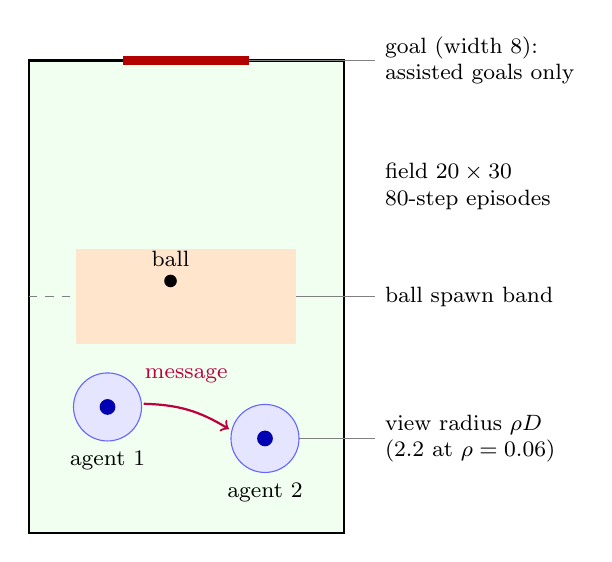
\begin{tikzpicture}[scale=0.2,font=\footnotesize]
  % field
  \fill[green!6] (0,0) rectangle (20,30);
  \draw[thick] (0,0) rectangle (20,30);
  \draw[dashed,gray] (0,15) -- (20,15);
  \fill[orange!20] (3,12) rectangle (17,18);
  \draw[line width=3pt,red!70!black] (6,30) -- (14,30);
  % agents and view circles (radius rho*D = 2.16)
  \draw[blue!60,fill=blue!10] (5,8) circle (2.16);
  \fill[blue!70!black] (5,8) circle (0.5);
  \node[below] at (5,5.8) {agent 1};
  \draw[blue!60,fill=blue!10] (15,6) circle (2.16);
  \fill[blue!70!black] (15,6) circle (0.5);
  \node[below] at (15,3.8) {agent 2};
  \fill (9,16) circle (0.4);
  \node[above] at (9,16.3) {ball};
  \draw[->,thick,purple] (7.3,8.2) to[bend left=15] (12.7,6.6);
  \node[purple] at (10,10) {message};
  % annotations to the right
  \draw[gray] (14,30) -- (22,30) node[right,black,align=left] {goal (width 8):\\assisted goals only};
  \draw[gray] (17,15) -- (22,15) node[right,black,align=left] {ball spawn band};
  \draw[gray] (17.16,6) -- (22,6) node[right,black,align=left] {view radius $\rho D$\\($2.2$ at $\rho=0.06$)};
  \node[right,align=left] at (22,22) {field $20\times30$\\80-step episodes};
\end{tikzpicture}
\caption{The environment to scale in the main regime. Each agent sees the ball and its teammate only
inside its circle. A message carries the sender's view of the ball, its position and its last touch.}
\label{fig:env}
\end{figure}

We built a small Gymnasium environment (Fig.~\ref{fig:env}). Two agents start in their own half and
the ball somewhere in midfield; the team attacks the goal at the top. Agents move in four directions,
boost forward or wait, and the ball can be dribbled. An episode lasts 80 steps and ends at the first
goal. Three design choices, each the outcome of an experiment in Section~\ref{sec:history}, make
communication matter:

\textbf{Assisted goals.} A goal counts only if the scorer's teammate touched the ball in the last 40
steps. Without this rule, one agent could score alone.

\textbf{Short sight.} An agent sees the ball or its teammate only within $\rho D$ of itself, where
$D$ is the field diagonal. At $\rho=0.06$ this is 2.2 units, much less than one kick, so most of the
time neither agent knows where the ball is. Each agent remembers where it last saw, or was told, the
ball and its teammate were.

\textbf{Messages with content.} A message reports what the sender sees: the ball's position and
velocity, the sender's own position and when it last touched the ball. It arrives after $\delta$
steps and stays visible for 10. Agents also observe how many messages they and their teammate have
left.

\textbf{Reward.} The team earns $+100$ per assisted goal, a small bonus for being near the ball and
two potential-based terms~\citep{ng1999}, which leave the optimal policy unchanged:
\begin{equation}
F_t=\Phi(s_{t+1})-\Phi(s_t)+\gamma\Psi(s_{t+1})-\Psi(s_t),
\end{equation}
where $\Phi$ rewards moving the ball toward the goal and the nearest agent toward the ball, and
$\Psi=20$ while a pass would make the next goal count. We always report goals, never shaped return.

% =====================================================================
\section{Method}\label{sec:method}
% =====================================================================

\subsection{Learners}

Each agent is an independent Double DQN (Eq.~\ref{eq:ddqn}) on a 45-dimensional observation, written in
NumPy with hand-coded backpropagation; for networks this small it trains several times faster on a
CPU than a deep-learning framework. Execution is fully decentralised. Table~\ref{tab:hparams} lists the
settings.

\begin{table}[!t]
\centering\small
\caption{Environment and training settings (main regime).}
\label{tab:hparams}
\begin{tabularx}{\linewidth}{@{}>{\raggedright\arraybackslash}p{0.27\linewidth}X@{}}
\toprule
Episode & 80 steps, ends at the first goal \\
View radius & $\rho=0.06$ of the diagonal (2.2 units) \\
Q-network & MLP 128--128, 3-step returns, $\gamma=0.99$ \\
Optimiser & Adam, lr $5\cdot10^{-4}$, batch 64 \\
Replay, target & buffer $10^5$, Polyak $\tau=0.005$ \\
Exploration & $\epsilon$ from 1 to 0.05 over 10\% of training \\
Message gate & MLP 64--64, cost $c=0.05$, horizon $H=40$ \\
Training & 15\,000 episodes, best of 60 snapshots \\
\bottomrule
\end{tabularx}
\end{table}

\subsection{Three ways to send}

The content of a message is fixed (the sender's current view), so the only choice is \emph{when} to
send. Three senders separate the questions:
\begin{itemize}
\item \cfg{F<B>}, \textbf{fixed schedule}: broadcast every $\lceil T/B\rceil$ steps, whatever the
sender sees. This measures the value of the information alone.
\item \cfg{R<B>}, \textbf{rule}: send when the sender sees the ball and its previous message has
expired; a sensible hand-coded trigger.
\item \cfg{L<B>}, \textbf{learned}: a message gate decides when to spend the budget.
\end{itemize}
\cfg{A} denotes no communication. The proposal's settings B, C and D correspond to \cfg{Linf}, a learned
sender limited to every 5th step, and \cfg{L20}.

\subsection{Learning when to send}\label{sec:gate}

The learned sender only considers sending when it can see the ball; otherwise it has nothing to
report. At those moments a small network $g_{\phi_i}$ scores how much a message is worth to the team,
and the agent sends if the score exceeds a cost $c$.

How should $g$ be trained? A message changes what the \emph{teammate} does, often many steps later,
so the sender's own reward says little about it. We therefore ask the simulator. At up to two random
decision points per episode the game is copied: in one copy the message is delivered, in the other it
is withheld. Both copies play on for $H=40$ steps with the current policies, and the gate learns the
difference in team reward:
\begin{equation}
A^i(o^i_t)=\sum_{h<H}\gamma^h\big(r^{\text{send}}_{t+h}-r^{\text{silent}}_{t+h}\big).
\label{eq:rollout}
\end{equation}
This is a difference reward computed from the team reward alone. Because the sending copy has one
message fewer left, it also accounts for the budget the message uses up. Copying the game is needed
only in training (centralised training, decentralised execution). As an ablation we keep the
proposal's idea of regressing the Monte-Carlo team return after each decision.

Early in training, a random sender teaches receivers to ignore messages. For the first 30\% of
training the rule therefore decides in the learned sender's place, with a probability fading from 1
to 0 (Algorithm~\ref{alg:train}).

\begin{algorithm}[!t]
\caption{Training a team with a learned sender}\label{alg:train}
\small
\begin{algorithmic}[1]
\For{each episode}
  \While{the episode is running}
    \For{each agent $i$}
      \State $a^i\gets\epsilon$-greedy action from $Q_{\theta_i}$
      \If{$i$ sees the ball and has budget left}
        \State $m^i\gets\ind[g_{\phi_i}(o^i)>c]$ \Comment{rule, early on}
        \If{this decision is sampled}
          \State copy the game; play on with
          \Statex \hspace{2.6em}and without $m^i$; store $(o^i,A^i)$
        \EndIf
      \EndIf
    \EndFor
    \State step; update each $Q_{\theta_i}$ and $g_{\phi_i}$
  \EndWhile
  \State every 250 episodes: validate, keep the best
\EndFor
\end{algorithmic}
\end{algorithm}

% =====================================================================
\section{How We Got Here}\label{sec:history}
% =====================================================================

The design above is the sixth version of the project. Table~\ref{tab:history} summarises the
1\,213 runs that led to it; every run's training history is in the repository. We describe them
because the failures explain the final design, and because they are a finding in themselves: the value
of communication turned out to be easy to hide.

\begin{table*}[!t]
\centering\small
\caption{Development iterations. Runs counts every trained team (one configuration, one seed).}
\label{tab:history}
\begin{tabularx}{\textwidth}{@{}l l r >{\raggedright\arraybackslash}X >{\raggedright\arraybackslash}X@{}}
\toprule
Ver. & Dates & Runs & What changed & What we saw \\
\midrule
v0 & Oct 19--Nov 3 & 114 & Proposal design: four message tokens, scripted keeper, 200-step episodes; sanity
runs, first sweep over $\rho\in\{1,0.75,0.5,0.25\}$ & DQN learns to score, but \cfg{A} already scores
92--95\% at $\rho\ge0.25$: one agent can score alone \\
v1 & Nov 4 & 105 & Assisted goals; keeper removed; views down to $\rho=0.15$ and $0.1$ &
Unlimited learned sender $+5.6$\,pp (n.s.); budgeted learned senders 11--18\,pp \emph{below} \cfg{A} \\
v2 & Nov 8--9 & 49 & Event-triggered learned sender; fixed-schedule baselines; best-snapshot selection
& Learned budgets still 11--47\,pp below \cfg{A} \\
v3 & Nov 9--11 & 568 & 80-step episodes; rule senders; send/silent gate with value-of-information
credit; rule handover; 10 seeds & No sender beats \cfg{A}; learned budget 10 is $-24.8$\,pp
($p=0.001$); the gain grows as the view shrinks \\
v4 & Nov 10--12 & 305 & Memory of last sightings; 10k episodes; medians and Mann--Whitney tests;
regime pilot & \cfg{A} scores 91--97\% at $\rho\ge0.1$ (ceiling); seeds collapse mid-training; at
$\rho=0.05$ nothing learns \\
v5 & Nov 18--20 & 72 & Code review fixes; rollout credit; pre-registered pilot & Gap opens: 26\% vs.\
71\% at $\rho=0.06$ \\
\midrule
Main & from Nov 21 & 580 & Regime fixed by the pilot; 10 seeds & Section~\ref{sec:results} \\
\bottomrule
\end{tabularx}
\end{table*}

\begin{figure*}[!t]
\centering
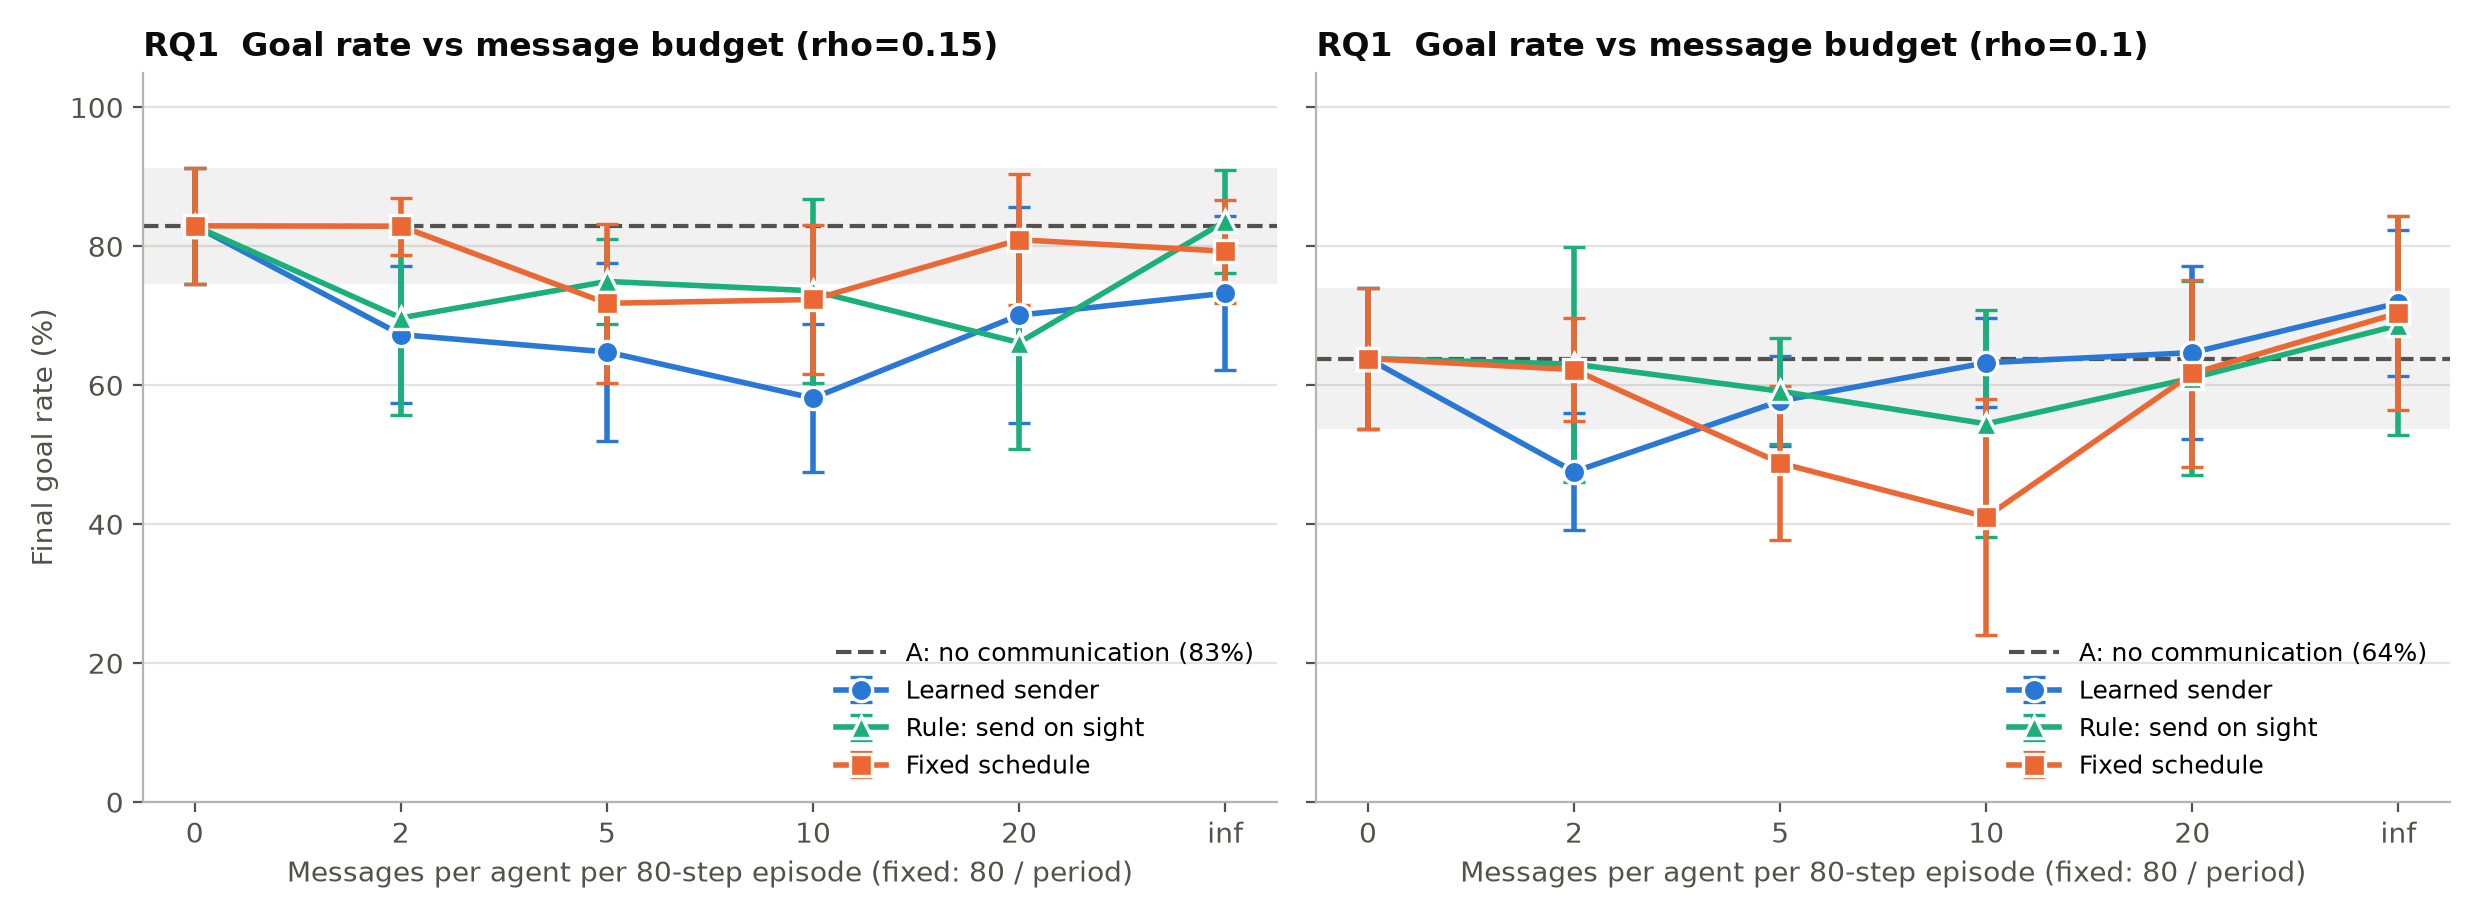
\includegraphics[width=0.9\textwidth]{figures/dev/v3_rq1_budget.png}
\caption{v3 (510 runs, 10 seeds): goal rate against the message budget (mean and 95\% CI). No sender
beats no communication (dashed), and the learned sender at small budgets does worse.}
\label{fig:v3}
\end{figure*}

\textbf{v0--v2: making communication necessary.} The proposal's design gave the agents four abstract
tokens (attack, defend, pass, rotate) and a scripted goalkeeper. Sanity runs confirmed that DQN learns
to score, but the first sweep showed that a single agent could score on its own, so a teammate's
information was worthless. Against the keeper the task did not learn at all. We removed the keeper and
added the assist rule, and later made the learned sender event-triggered: it decides only when it sees
the ball, so every message has something to report. Still, budgeted learned senders scored 11--47
points \emph{below} the team that never spoke.

\textbf{v3: a large sweep with a negative answer.} Two changes made the task harder: 80-step
episodes, because with 200 steps nearly every team eventually scored, and a hand-coded rule sender as
a reference. The learned sender now chose only between sending and staying silent; picking among
interchangeable tokens had fed the receiver a drifting input. Its credit was the improvement a
message made to the receiver's own Q-values. Over 510 runs with 10 seeds, no sender beat \cfg{A}
(Fig.~\ref{fig:v3}). One trend held, however: communication helped more as the view shrank
(Fig.~\ref{fig:v3rho}). At $\rho=0.1$ all three unlimited senders beat \cfg{A}; at full view all lost.
This suggested that the effect was real but masked.

\begin{figure}[!t]
\centering
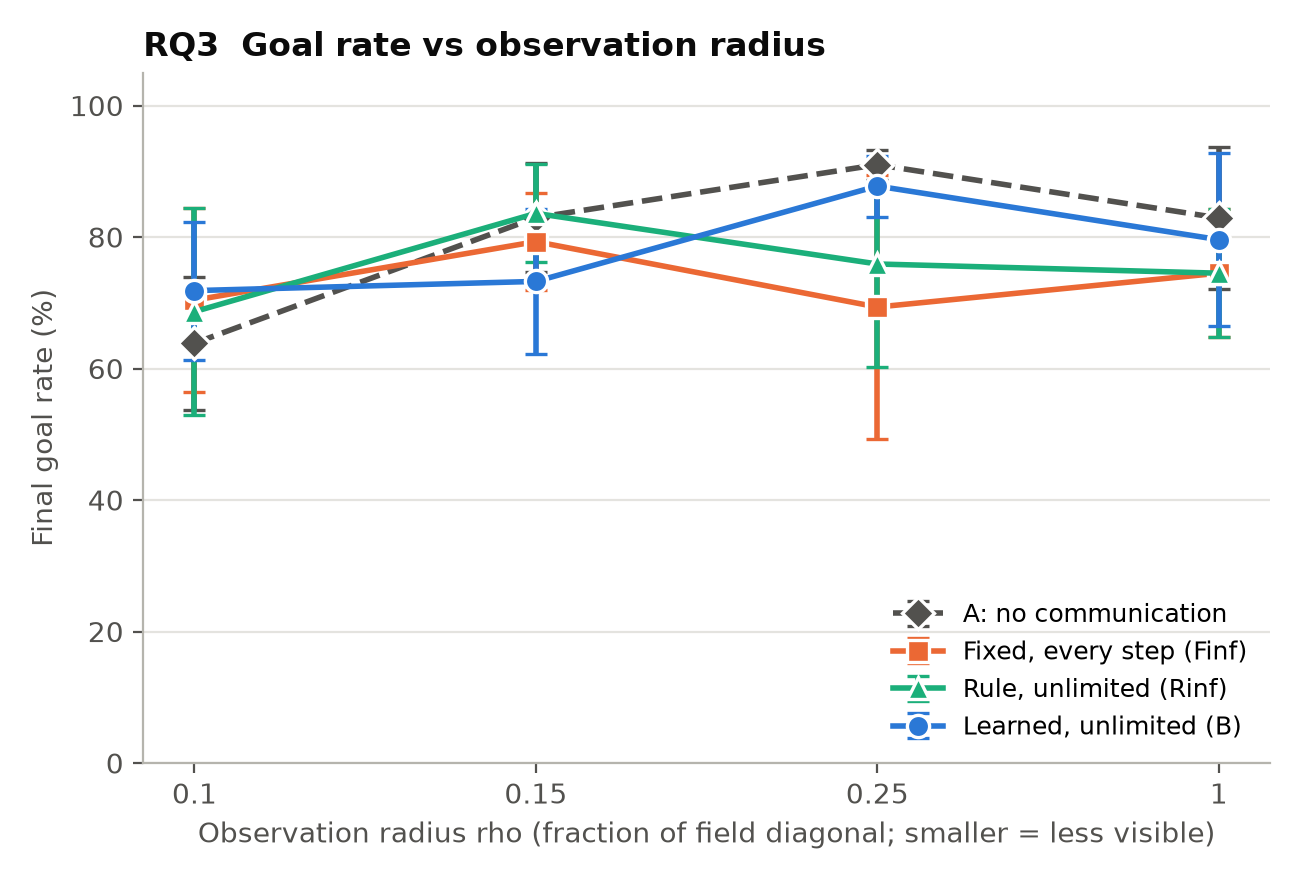
\includegraphics[width=0.95\linewidth]{figures/dev/v3_rq3_observability.png}
\caption{v3: goal rate against the view radius $\rho$. Communication only pays off when agents see
little ($\rho=0.1$, left).}
\label{fig:v3rho}
\end{figure}

\textbf{v4: a ceiling and collapsing seeds.} Agents gained a memory of their last sightings, so a
message is not forgotten after 10 steps, and training was extended to 10\,000 episodes. With memory,
however, \cfg{A} scored 91--97\% at every $\rho\ge0.1$, which left no room for messages to help.
Learning curves also revealed that teams often reached 80--90\% and then collapsed
(Fig.~\ref{fig:v4}), so a single bad seed could dominate a mean; we switched to medians and
Mann--Whitney tests. A small regime pilot showed that at $\rho=0.05$ no team learned reliably.

\begin{figure*}[!t]
\centering
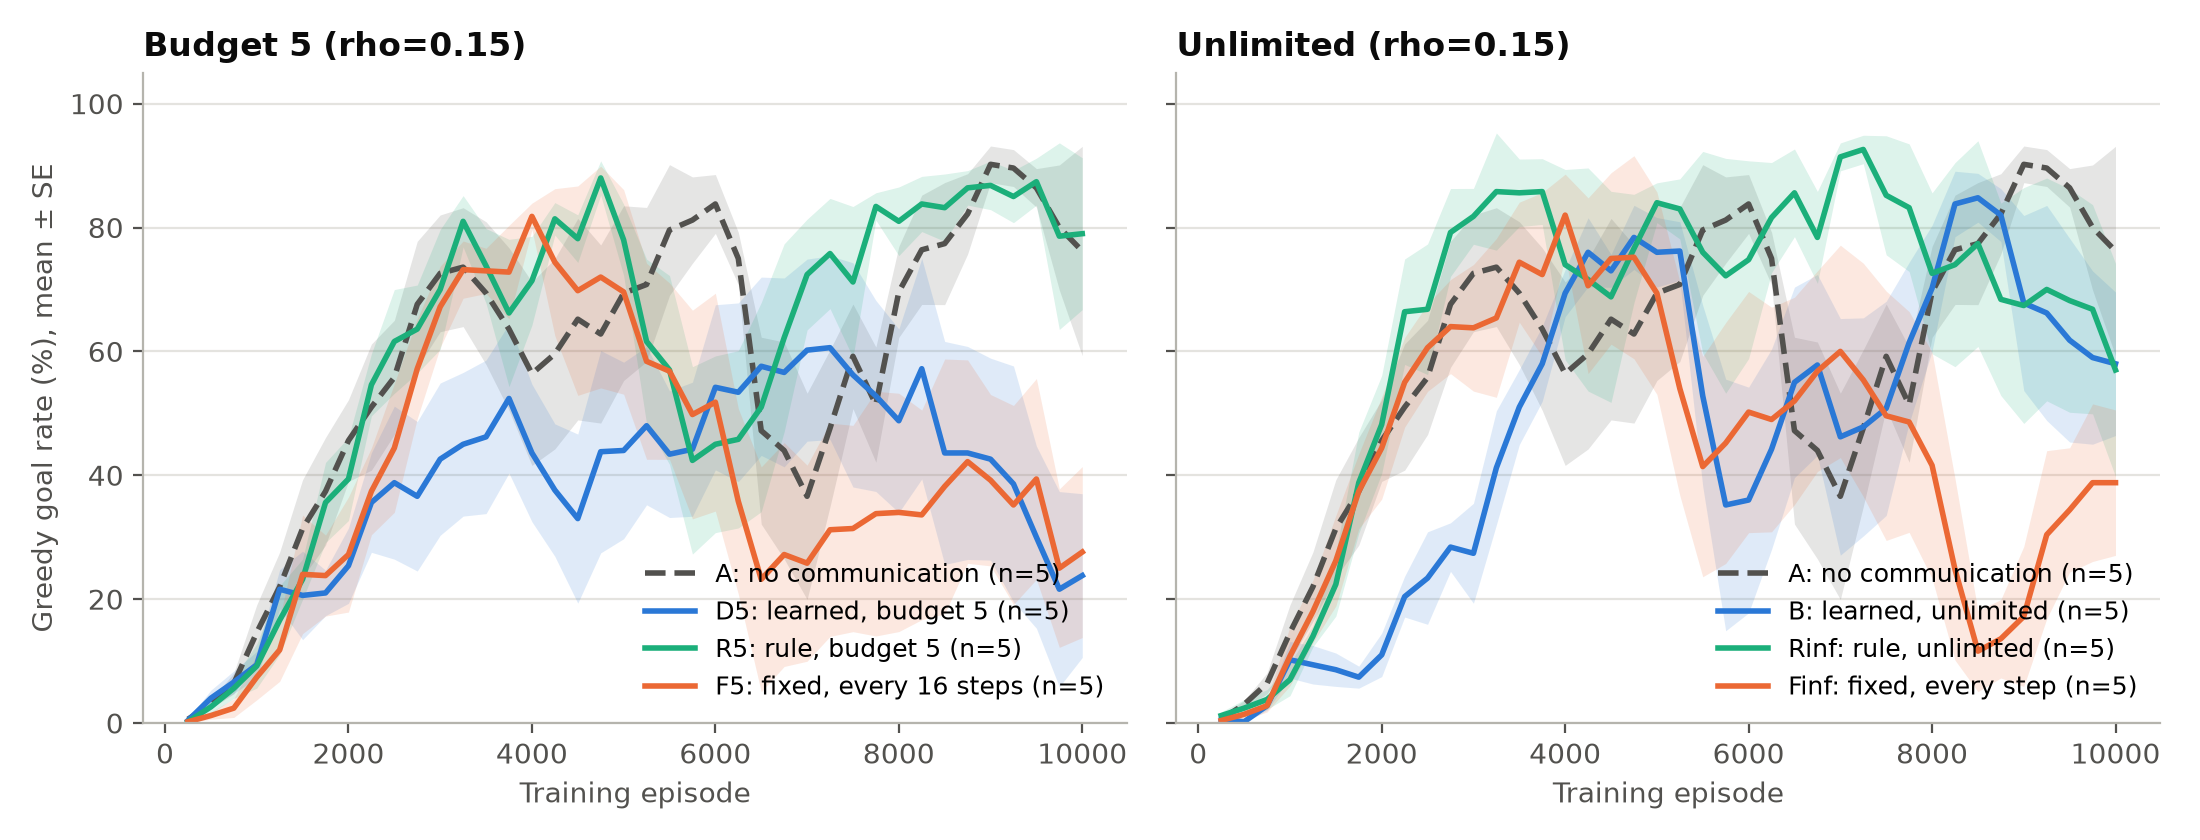
\includegraphics[width=0.9\textwidth]{figures/dev/v4_learning_curves.png}
\caption{v4: validation goal rate during training at $\rho=0.15$ (mean $\pm$ SE, 5 seeds). Teams
reach 80--90\% and then collapse, which best-snapshot selection hides.}
\label{fig:v4}
\end{figure*}

\textbf{v5: the review.} We then reviewed the code against the saved runs and checked each suspected
flaw on trained policies. Three findings explained the earlier results:
\begin{itemize}
\item \textbf{A free channel.} An assist flag in the observation revealed the teammate's true touches to
every team, including \cfg{A}. Clearing it changed \cfg{A}'s action in 64\% of the steps where it was
set: the ``silent'' team had been communicating all along.
\item \textbf{A credit that could not be negative.} The receiver's Q-value change never penalised a
wasted message and was uncorrelated with a message's effect on the outcome. We replaced it with the
rollout credit of Section~\ref{sec:gate}.
\item \textbf{Hidden instability.} 26 of 98 v4 runs ended training below 50\% goals, but only 6 did after
best-snapshot selection. We now report the final policy as well.
\end{itemize}
Smaller fixes followed: the time limit is terminal because the remaining time is observed, messages
report the sender's view at decision time, and the networks became 5--8$\times$ faster.

\textbf{The pre-registered pilot.} Many choices, the view radius above all, could be tuned until
communication looks good. To avoid this, we wrote the decision rules down \emph{before} a 72-run pilot
on seeds disjoint from the main sweep (Table~\ref{tab:pilot}). The regime rule chose the largest
relative gap between \cfg{A} and an every-step broadcast among regimes where both still learn:
$\rho=0.06$, at 26\% vs.\ 71\%. At $\rho=0.075$ the gap was already clear (Fig.~\ref{fig:pilot}),
and the rule sender matched the broadcast's 83\% with only 2 messages per episode instead of 47, a
first hint that a small budget suffices.

\begin{table}[!t]
\centering\small
\caption{Pilot decisions (rules fixed in advance; 3 seeds).}
\label{tab:pilot}
\begin{tabularx}{\linewidth}{@{}>{\raggedright\arraybackslash}p{0.22\linewidth}X@{}}
\toprule
Question & Decision (evidence) \\
\midrule
Share weights & no: sharing 6\,pp worse on \cfg{Finf} \\
Regime & single goal, $\rho=0.06$: \cfg{A} 26\% vs.\ \cfg{Finf} 71\% \\
Gate credit & rollout: \cfg{L4} 69\% vs.\ 64\% (team return) \\
Length & 15\,000 episodes: curves flat by then \\
LR decay & off: 7\% of runs unstable (rule: $>$10\%) \\
\bottomrule
\end{tabularx}
\end{table}

\begin{figure}[!t]
\centering
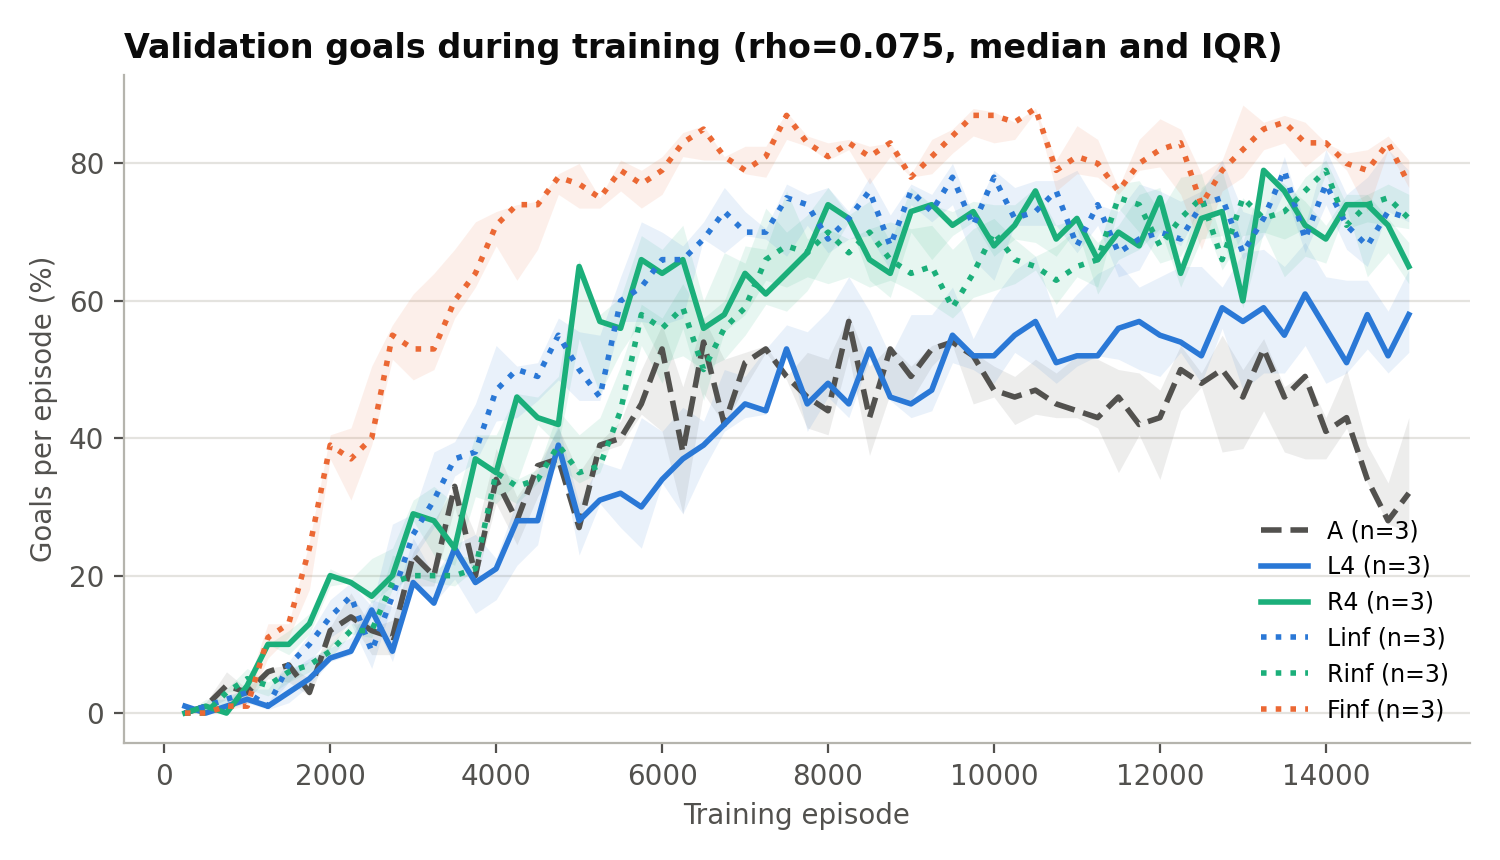
\includegraphics[width=\linewidth]{figures/dev/pilot_learning_curves.png}
\caption{v5 pilot at $\rho=0.075$ (median and IQR, 3 seeds): with the free channel removed,
communicating teams clearly beat \cfg{A}, which plateaus near 50\%.}
\label{fig:pilot}
\end{figure}

Relative to the proposal, the iterations thus led to assisted goals and no opponent, messages that
carry observations rather than abstract tokens, rollout credit instead of DQN for the message
decision, and the rule and fixed senders as reference points.

% =====================================================================
\section{Main Experiment}\label{sec:setup}
% =====================================================================

\begin{figure*}[!t]
\centering
\resultfig[0.9\textwidth]{rq1_budget.png}{3.2cm}\\[2pt]
{\small (a) RQ1: goal rate against the message budget}\\[6pt]
\resultfig[0.9\textwidth]{rq3_observability.png}{3.2cm}\\[2pt]
{\small (b) RQ3: goal rate and communication gain against the view radius}
\caption{Main sweep at $\rho=0.06$, 10 seeds. (a) Learned, rule and fixed senders against the budget
(median and IQR; dashed: \cfg{A}), with fitted saturation curves. (b) \cfg{A}, \cfg{Linf} and
\cfg{Rinf} against $\rho$ (left) and the gain $\Delta(\rho)$ with 95\% bootstrap CI (right).}
\label{fig:main}
\end{figure*}

Every configuration of the main sweep is trained with 10 seeds in the regime fixed by the pilot
(Table~\ref{tab:sweep}), 580 runs in total. A run takes 30--40 minutes on one core, so the sweep needs
about 300--400 core-hours, roughly 50 hours of wall-clock time on the machine used.

\begin{table}[!t]
\centering\small
\caption{Main sweep: 58 configurations $\times$ 10 seeds.}
\label{tab:sweep}
\begin{tabularx}{\linewidth}{@{}c>{\raggedright\arraybackslash}Xl@{}}
\toprule
& Configurations & Question \\
\midrule
1 & \cfg{A}; \cfg{L}, \cfg{R} at $B\in\{1,\dots,24,\infty\}$; \cfg{F} at 6 rates & RQ1 \\
2 & delays $\delta\in\{1,2,4,8\}$; \cfg{L} without budget features & RQ2 \\
3 & \cfg{A}, \cfg{Linf}, \cfg{Rinf} at five wider $\rho$ & RQ3 \\
4 & proposal setting \cfg{C}; team-return credit & ablation \\
\bottomrule
\end{tabularx}
\end{table}

\textbf{Evaluation.} Every 250 episodes the greedy policy is scored on 100 fixed episodes; the best
snapshot and the final policy are then tested on 200 unseen episodes. We report medians with
interquartile ranges (IQR) over seeds, Holm-corrected Mann--Whitney tests and Spearman correlations
for trends. For the saturation point we fit $y(B)=y_\infty-(y_\infty-y_0)e^{-B/\beta}$ and report
$B_{90}=\beta\ln10$, the budget that recovers 90\% of the gain from unlimited communication, with a
bootstrap interval over seeds. A random team and a hand-coded team serve as reference points.

% =====================================================================
\section{Results}\label{sec:results}
% =====================================================================

\subsection{Learning and reference teams}

\todo{Main sweep running. Fill Table~\ref{tab:main} from \cfg{checkpoints/sweep\_v5/results.md}. Do
the trained teams beat the random and hand-coded teams? How far apart are the best snapshot and the
final policy?}

\begin{table}[!t]
\centering\small
\caption{Goal rate (\%) at $\rho=0.06$: median [IQR] over 10 seeds.}
\label{tab:main}
\begin{tabular}{@{}lccc@{}}
\toprule
Team & Best & Final & Msgs/agent \\
\midrule
Random & \pend & -- & 0 \\
Hand-coded & \pend & -- & 0 \\
Hand-coded + rule msgs & \pend & -- & \pend \\
\cfg{A} (no messages) & \pend & \pend & 0 \\
\cfg{Finf} (every step) & \pend & \pend & \pend \\
\cfg{Rinf} (rule) & \pend & \pend & \pend \\
\cfg{Linf} (learned) & \pend & \pend & \pend \\
\bottomrule
\end{tabular}
\end{table}

\begin{figure}[!t]
\centering
\resultfig{learning_curves.png}{3.6cm}
\caption{Validation goal rate during training at $\rho=0.06$ (median and IQR, 10 seeds).}
\label{fig:curves}
\end{figure}

\subsection{RQ1: when do more messages stop helping?}

\todo{Where does each curve in Fig.~\ref{fig:main}a flatten, and does the learned sender saturate
earlier than the fixed schedule? Report $B_{90}$ per sender (Table~\ref{tab:rq1}), the drop when message
content is shuffled, and when in the episode learned agents send.}

\begin{table}[!t]
\centering\small
\caption{Saturation budget per sender: fitted $B_{90}$ [95\% CI], the smallest tested budget at 90\% of
the gain, and Spearman's $\rho_s$ against $B$.}
\label{tab:rq1}
\begin{tabular}{@{}lccc@{}}
\toprule
Sender & $B_{90}$ & Smallest $B$ & $\rho_s$ \\
\midrule
Learned (\cfg{L}) & \pend & \pend & \pend \\
Rule (\cfg{R}) & \pend & \pend & \pend \\
Fixed (\cfg{F}) & \pend & \pend & \pend \\
\bottomrule
\end{tabular}
\end{table}


\subsection{RQ2: delay}

\todo{At which delay does communication stop beating \cfg{A}? Spearman trend against $\delta$.}

\begin{figure}[!t]
\centering
\resultfig{rq2_delay.png}{3.6cm}
\caption{RQ2: goal rate of \cfg{Linf} and \cfg{Rinf} against the delivery delay $\delta$.}
\label{fig:rq2}
\end{figure}

\subsection{RQ3: observability}

\todo{Does the gain $\Delta(\rho)$ in Fig.~\ref{fig:main}b grow as $\rho$ shrinks (slope against $\log\rho$ with CI), as v3
suggested? Does $B_{90}$ move between $\rho=0.06$ and $0.1$? Also report the credit ablation
(\cfg{L4}, rollout vs.\ team return).}

\FloatBarrier

% =====================================================================
\section{Limitations and Conclusion}
% =====================================================================

Independent learners have no convergence guarantee, which is why we report the final policy next to
the selected one. The rollout credit needs a simulator that can be copied during training. Messages
have a fixed content, so we study the timing of communication under a budget, not emergent language.
There is no opponent, so the results concern coordination between teammates only.

The longest part of this project was making communication \emph{measurable}. Its value was hidden
first by a task one agent could solve alone, then by a ceiling, by a free channel through the
observation, and by a credit that could not penalise waste. With those removed, a hand-coded sender
already matches an every-step broadcast with a few messages per episode. \todo{One or two sentences
on the main sweep's answer to RQ1--RQ3.}

% =====================================================================
\section*{Contributions}
% =====================================================================

\begin{table}[h]
\centering\small
\begin{tabularx}{\linewidth}{@{}l>{\raggedright\arraybackslash}Xc@{}}
\toprule
Member & Assigned tasks & Done \\
\midrule
Aryan Kumar & Environment; system integration & \todo{?} \\
Rayan Talukder & DQN and message agents; replay buffer; training loop & \todo{?} \\
S.\ A.\ Gantedi & Experiment runner; metrics; plots and analysis & \todo{?} \\
K.\ V.\ K.\ Reddy & Literature review; report writing and proofreading & \todo{?} \\
\bottomrule
\end{tabularx}
\end{table}

\textbf{Code.} Code, pilot rules and the training history of every run:
\url{https://github.com/AceAryan/marl-rocket}.

% =====================================================================
\small
\begin{thebibliography}{99}
\setlength{\itemsep}{1pt}
\bibitem{weiss2000} G.~Weiss. \emph{Multiagent Systems: A Modern Approach to Distributed Artificial
Intelligence}. MIT Press, 2000.
\bibitem{zhang2013} C.~Zhang and V.~Lesser. Coordinating multi-agent reinforcement learning with
limited communication. In \emph{AAMAS}, 2013.
\bibitem{sukhbaatar2016} S.~Sukhbaatar, A.~Szlam, and R.~Fergus. Learning multiagent communication
with backpropagation. In \emph{NeurIPS}, 2016.
\bibitem{foerster2016} J.~Foerster, I.~A.~Assael, N.~de~Freitas, and S.~Whiteson. Learning to
communicate with deep multi-agent reinforcement learning. In \emph{NeurIPS}, 2016.
\bibitem{singh2019} A.~Singh, T.~Jain, and S.~Sukhbaatar. Learning when to communicate at scale in
multiagent cooperative and competitive tasks. In \emph{ICLR}, 2019.
\bibitem{oliehoek2016} F.~A.~Oliehoek and C.~Amato. \emph{A Concise Introduction to Decentralized
POMDPs}. Springer, 2016.
\bibitem{watkins1992} C.~J.~C.~H.~Watkins and P.~Dayan. Q-learning. \emph{Machine Learning},
8(3--4):279--292, 1992.
\bibitem{mnih2015} V.~Mnih, K.~Kavukcuoglu, D.~Silver, et al. Human-level control through deep
reinforcement learning. \emph{Nature}, 518(7540):529--533, 2015.
\bibitem{tan1993} M.~Tan. Multi-agent reinforcement learning: Independent vs.\ cooperative agents.
In \emph{ICML}, 1993.
\bibitem{vanhasselt2016} H.~van Hasselt, A.~Guez, and D.~Silver. Deep reinforcement learning with
double Q-learning. In \emph{AAAI}, 2016.
\bibitem{sutton2018} R.~S.~Sutton and A.~G.~Barto. \emph{Reinforcement Learning: An Introduction}.
MIT Press, 2nd edition, 2018.
\bibitem{rashid2018} T.~Rashid, M.~Samvelyan, C.~Schroeder de Witt, G.~Farquhar, J.~Foerster, and
S.~Whiteson. QMIX: Monotonic value function factorisation for deep multi-agent reinforcement
learning. In \emph{ICML}, 2018.
\bibitem{wolpert2002} D.~H.~Wolpert and K.~Tumer. Optimal payoff functions for members of
collectives. \emph{Advances in Complex Systems}, 4(2--3):265--279, 2001.
\bibitem{ng1999} A.~Y.~Ng, D.~Harada, and S.~Russell. Policy invariance under reward transformations:
Theory and application to reward shaping. In \emph{ICML}, 1999.
\end{thebibliography}

\end{document}
